% Esport Language (PaRa) , first experiments
% This is a rapid prototype for planning Pasigraphy Rhapsody (Paszigráfia Rapszódia, PaRa)
%
% con_prel_para.tex
%
% Copyright (C) 2019 Norbert Bátfai, nbatfa@gmail.com, batfai.norbert@inf.unideb.hu
%
%  This program is free software: you can redistribute it and/or modify
%  it under the terms of the GNU General Public License as published by
%  the Free Software Foundation, either version 3 of the License, or
%  (at your option) any later version.
%
%  This program is distributed in the hope that it will be useful,
%  but WITHOUT ANY WARRANTY; without even the implied warranty of
%  MERCHANTABILITY or FITNESS FOR A PARTICULAR PURPOSE.  See the
%  GNU General Public License for more details.
%
%  You should have received a copy of the GNU General Public License
%  along with this program.  If not, see <https://www.gnu.org/licenses/>.
%
% Version history
%
% Initial hack
%
% con_prel_para.tex
% Working title: Construction of the Language of the Esports Culture: A Preliminary Study
%
\documentclass[a4paper]{article}
\usepackage{preamble}
\usepackage[letterspace=290]{microtype}
\usepackage{tcolorbox}
\usepackage{minted}
\usepackage{csquotes}
\usepackage{shellesc}

\tcbuselibrary{skins}
\tcbuselibrary{minted}

%
% The following code is based on the
% Thomas F. Sturm, The tcolorbox package Manual for version 4.20 (2019/03/02)
% http://www.ctan.org/pkg/tcolorbox
%
\newtcblisting{prologbox}{
listing engine=minted,
minted language=prolog,
minted options={breaklines,autogobble,linenos,numbersep=3mm},
colback=green!5!white,colframe=red!75!black,listing only,
left=5mm,enhanced,
overlay={\begin{tcbclipinterior}\fill[red!20!yellow!20!white] (frame.south west)
rectangle ([xshift=5mm]frame.north west);\end{tcbclipinterior}}}
%
% The following code is based on the
% Thomas F. Sturm, The tcolorbox package Manual for version 4.20 (2019/03/02)
% http://www.ctan.org/pkg/tcolorbox
%
\tcbset{frogbox/.style={enhanced,
enlarge top by=6mm,
overlay={\foreach \x in {9cm,10.2cm} {
\begin{scope}[shift={([xshift=\x, yshift=-.04cm]frame.north west)}]
\path[draw=red!65!black,fill=red!10,line width=.6mm] (0,0) arc (-20:200:5mm);
\path[fill=black] (-0.51,.0) arc (-50:240:2mm);
\path[fill=white] (-0.64,.1) arc (0:360:.4mm);
\end{scope}}}}}

\newcommand{\parafop}[3]{
\begin{tcolorbox}[
colupper=red!50!black,colback=red!5!white,
colframe=red!75!black,
colbacktitle=yellow!50!red,
coltitle=red!25!black,
fonttitle=\bfseries,
subtitle style={boxrule=0.4pt,
colback=yellow!50!red!25!white} ]
\tcbsubtitle{{#1}}
{#2}
\tcbsubtitle{{#3}}
\end{tcolorbox}
}

\newcommand{\parafopp}[4]{
\begin{tcolorbox}[
colupper=red!50!black,colback=red!5!white,
colframe=red!75!black,
colbacktitle=yellow!50!red,
coltitle=red!25!black,
fonttitle=\bfseries,
subtitle style={boxrule=0.4pt,
colback=yellow!50!green!25!white} ]
\tcbsubtitle{{#1}}
{#2}
\tcbsubtitle{{#3}}
{\lstinline[language=Prolog]!#4!}
\end{tcolorbox}
}

\newcommand{\parafopt}[4]{
\begin{tcolorbox}[
title={{#1}},
coltitle=red!25!black,
colbacktitle=white!60!red,
colupper=red!50!black,
colback=red!5!white,
colframe=red!75!black,
fonttitle=\bfseries,
subtitle style={boxrule=0.4pt,
colback=yellow!50!red!25!white,
coltitle=red!60!black}]
\tcbsubtitle{{#2}}
{#3}
\tcbsubtitle{{#4}}
\end{tcolorbox}
}

\begin{document}

\begin{titlepage}
\pagecolor{cyan}
\vspace*{\fill}
	\centering

	{\color{gray!10!white}\Huge\bf ESPORT NYELV}
	\\
	\vspace{.2cm}
	{\color{black!80!white}\Large\lsstyle \  Paszigráfia Rapszódia}
	\vspace{1cm}

	\begin{tikzpicture}[thick, scale=2, every node/.style={scale=2}]
\prelparaIIID{1}{"3:4:3:0:1:2:2:3:4:10:2:0:9:9:0:8:2:1:6:6:1:6:2:1:5:5:1:8:2:1:7:7:1:4:2:1:3:3:1:4:2:1:3:3:1:10:2:1:7:7:1:6:2:1:5:5:1"}
\prelparaIIID{2} {"4:4:3:1:2:2:2:3:4:10:2:0:9:9:0:8:2:1:6:6:1:6:2:1:5:5:1:8:2:1:7:7:1:4:2:1:3:3:1:4:2:1:3:3:1:2:1:1:1:6:2:1:5:5:1:4:1:1:1:8:2:2:2:4:4:2:1:1:1"}
\prelparaIIID{1}{"3:4:3:0:1:2:2:3:4:10:2:0:9:9:0:8:2:1:6:6:1:6:2:1:5:5:1:8:2:1:7:7:1:4:2:1:3:3:1:4:2:1:3:3:1:10:2:1:7:7:1:6:2:1:5:5:1"}
\end{tikzpicture}

\vspace{1cm}

	{\color{black!80!white}\Large\textls[655]{Pasigraphy Rhapsody}}
\\
	\vspace{.2cm}
	{\color{gray!10!white}\Huge\bf ESPORTS LANGUAGE}
\vspace*{\fill}
	\end{titlepage}


\title{Az esport kult\'ura nyelve\\{\large PaRa programozói kézikönyv}
\\The Language of the Esports Culture\\{\large PaRa Programmer's Guide}
}
\author{
	Bátfai Norbert\\
	\texttt{batfai.norbert@inf.unideb.hu}\\
    Információ Technológia Tanszék, Debreceni Egyetem\\
	\and
	Bátfai N\'andor Benj\'amin\\
	\texttt{batfai.nandi@gmail.com}\\
    Debreceni Egyetem Kossuth Lajos Gyakorló Általános Iskola\\
	}
\date{
    \today
}
\pagecolor{white}

\maketitle

\begin{abstract}
A Paszigráfia Rapszódia \cite{PARAREPO}, vagy röviden PaRa egy olyan mesterséges nyelv kialakítására törekv\H o kezdeményezés, mely lehet\H ové teszi a homunkulusz és a mesterséges homunkulusz közötti kommunikációt, ergó ez az esport kultúra nyelve \cite{MITEL}. A PaRa nyelvi mondatok el\H o\'all\'it\'as\'anak els\H o l\'ep\'ese a term\'eszetes nyelvi mondatok \'at\'ir\'asa egy els\H o\-ren\-d\H u logikai (FOL) nyelvre, melyb\H ol a PaRa mondat el\H o\'all\'it\'asa m\'ar auto\-ma\-ti\-z\'al\-ha\-t\'o \cite{CONPARA}. Ez a dokumentum a FOL nyelvi for\-d\'i\-t\'as\-ban \'es az erre \'ep\H ul\H o automatiz\'al\'ast t\'amogat\'o szoftverek haszn\'alat\'aban seg\'iti a leend\H o PaRa fejleszt\H oket.
\end{abstract}

\begin{otherlanguage}{english}
\begin{abstract}
The Pasigraphy Rhapsody \cite{PARAREPO}, or shortly PaRa (from it's Hungarian name Paszigr\'afia Rapsz\'odia) is an initiative to develop an artificial language that is intended to allow communication between the Homunculus and the Artificial Homunculus, ergo, it is the language of the esport culture \cite{MITEL}. The first step of the production of PaRa sentences is to translate natural language sentences to First-Order Logic (FOL) sentences from which the PaRa sentences can be produced automatically \cite{CONPARA}. This document helps future developers in FOL translating and in using automation software based on it.
\end{abstract}
\end{otherlanguage}

\newpage
\tableofcontents

\section{Bevezetés}

Az esport kultúra a donaldi \cite{Donald01} epizodikus, mimetikus, mitikus és teoretikus kultúrális szintek elképzelt következő fázisa \cite{MITEL}, \cite{SMNIST}. A teoretikus szinten kifejlődhetett a neumanni értelemben vett \textquote{önreprodukáló automata}, a központi idegrendszerrel és az emberi kultúrával, mint hordozóval összemérhető bonyolultságú értelmező program, a homunkulusz, amelyet mindannyian, mint a saját tudatunkat tapasztalunk meg. Amikor mesterséges intelligenciát szeretnénk létrehozni, akkor ezt a folyamatot akarjuk megismételni, ezért tekinthetjük ezt úgy, hogy a homunkulusz törekszik egy mesterséges homunkulusz kialakítására. Ezzel ennek a donaldi víziónak szeretnénk megfelelni: \textquote{az elme új architektúráját építjük meg, olyat, amely hatékonyabb reprezentációs eszközökkel rendelkezik, és képes saját magát megérteni} \cite[328]{Donald01}.

Miért kellene ehhez egy új donaldi átmenet? A matematikában, az emberiség legstabilabbnak tartott építményében felbukkanó ellentmondások kapcsán elindult kutatások egyértelművé tették, hogy a mitikus (beszélt nyelvi) kultúra szintjén ezeket nem lehet feloldani. Az elméleti kultúra szintjén, a matematikai logika nyelvén lehet egyáltalán érdemben beszélni róluk. Lássuk konkrét példákat is ellentmondásokra!
A \cite{ALBERT} könyvet követve a következő két antinómiát mutatjuk be: ha még  nem vagy benne a logikában, akkor az Evbulid paradoxont (kék pirula\footnote{Ha nem tudod, mi a kék és mi a piros pirula, akkor ideje megnézni a Mártix című mozit!}) olvasd most csak el, jópár hét múlva gyere lapozz vissza

\begin{tcolorbox}[
title={Evbulid paradoxon, i.e. IV. sz\'azad},
colupper=blue!50!black,
colback=blue!5!white,
colframe=blue!75!black,
colbacktitle=white!75!blue,
coltitle=blue!30!black,
fonttitle=\bfseries,
subtitle style={boxrule=0.4pt,
colback=yellow!50!blue!25!white} ]
Azt mondom: \textquote{\bf Hazudok.} K\'et lehet\H os\'eg van:
\begin{itemize}
\item Ha igazat mondok (nem hazudok), akkor hazudok.
\item Ha hazudok (hazudom, hogy hazudok), akkor igazat mondok.
\end{itemize}
\cite[183]{ALBERT}
\end{tcolorbox}


a Russel antinómia bemutatására (piros pirula\footnote{Jóval polulárisabban, mondjuk egy algebra kurzus szintjén azt mondanánk, hogy Cantor \'ota vannak ugye a halmazok, például a $H=\{1,2,3\}$ és általában bármely összességet tekinthetünk halmaznak. Ennek a $H$ halmaznak egy tulajdonsága, hogy elemk\'ent önmagát nem tartalmazza, azaz $H \notin H$. Vegy\"uk most az \"osszes halmazok halmaz\'at, mivel ez minden halmazt tartalmaz, így önmagát is, azaz feltéve, hogy $A$-val jelöljük, ez a tulajdonság jellemzi: $A \in A$. Majd tekintsük azt a halmazt, amely az összes ilyen tulajdonsággal nem rendelkező halmazt tartalmazza, tehát azokat, amelyek önmagukat elemként nem tartalmazzák, jelölésében legyen ez a $D$ halmaz. Kérdés, hogy $D$ eleme-e $D$-nek, tehát önmagát tartalmazza-e elemként? \begin{itemize}
\item $D \in D \Rightarrow D \notin D$
\item $D \notin D \Rightarrow D \in D$
\end{itemize}
\cite[16]{Szendrei}
})!


\begin{tcolorbox}[
title={Russel paradoxon, i.sz. XX. sz\'azad},
colupper=red!50!black,
colback=red!5!white,
colframe=red!75!black,
colbacktitle=white!75!red,
coltitle=red!30!black,
fonttitle=\bfseries,
subtitle style={boxrule=0.4pt,
colback=yellow!50!red!25!white} ]
Az $M^+$ na\'iv halmazelm\'elet form\'alis axiomatikus elm\'eletben a
$\forall z ( z\in \{y\vert \varphi(y) \} \equiv \varphi(z))$ absztrakci\'o axi\'om\'ab\'ol kiindulva, a $\varphi(z)=\neg (z \in z)$ absztrakci\'ot alkalmazva
\[
M^+ \vdash \forall z (z \in \{x\vert x\notin x\} \equiv z \notin z)
\]
amib\H ol a $\{x\vert x\notin x\}$ Russel halmazr\'ol a
\[
M^+ \vdash \{x\vert x\notin x\} \in \{x\vert x\notin x\} \equiv \{x\vert x\notin x\} \notin \{x\vert x\notin x\}
\]
t\"orv\'eny vezethet\H o le.

Viszont puszt\'an abb\'ol, hogy $\vDash \neg ( A \equiv \neg A)$ vagy a $\{x\vert x\notin x\} \in \{x\vert x\notin x\} \equiv \{x\vert x\notin x\} \notin \{x\vert x\notin x\}$ formula tagad\'as\'at tov\'abb alak\'itva (az $M^+$ logikai axi\'om\'ait felhaszn\'alva) kapjuk, hogy
\[
M^+ \vdash \neg (\{x\vert x\notin x\} \in \{x\vert x\notin x\} \equiv \{x\vert x\notin x\} \notin \{x\vert x\notin x\})
\]
Ezzel az ekvivalenciát és annak tagadását is levezettük az $M^+$ elm\'eletben, tehát az $M^+$ elm\'elet nem ellentmond\'asmentes. Ez a Russel antin\'omia \cite[182]{ALBERT}.
\end{tcolorbox}

Mi persze nem a matematika megalapozása körüli csatákba történő bekapcsolódásra gyúrunk, hanem egy univerzális mesterséges nyelvet szeretnénk széles körben elterjeszteni. Ezért a legjobb fegyverünkhöz nyúlunk, ami van: a matek legősibb, de mai formájában legmodernebb ágához, a matematikai logikához. Ezzel most egyetemeken találkoznak a matematikus és informatikus hallgatók. A donaldi idézett vízió megvalósításához ezen megtanulni beszélni az első lépés a mi olvasatunkban. S mivel az egyetem egy nyelv szempontjából nem tömegbázis, a megtanulásának és a modern matematikai gondolkodás elterjesztésének eszközei a tömegesen játszott elektronikus játékok lehetnek. Ez a Paszigráfia Rapszódia létrehozásának motivációja, hogy legyen egy olyan matematikai logikai alapú mesterséges, de természetesen a nemzeti anyanyelveinkre épülő nyelvünk, amely játékok alapjául is szolgálhat, s még egyben a tudomány egyetemes nyelve is lehet.

Az elektronikus játékok térnyerése egyértelmű tendencia, a szülő, nagyszülő nem érti mit jelent a játékfogyasztás megugrása vagy, hogy mi az esport. Talán nagy rendezettségű szellemi táplálék, amire a játékos agya mohón veti rá magát \cite{STHEOR}. Mindenesetre ha sikerülne PaRa alapú játékokkal tömeges szinten játszani, az az idézett donaldi vízió mentén olyan szinten fejleszthetné tovább az emberiség kognitív szintjét, amihez képes a nagyszülői esport \textquote{értetelenkedés} eltörpül.

\begin{otherlanguage}{english}
\section{Introduction}

The esports culture \cite{MITEL}, \cite{SMNIST} is a next imagined phase of Donald's \cite{Donald01} episodic, mimetic, mythic and theoretical stages of cognitive evolution.

\end{otherlanguage}

\subsection{Emberek, egerek, macskák és kutyák}

\begin{tcolorbox}[
frogbox,
coltitle=red!25!black,
colbacktitle=white!60!red,
title=Formalizálásos ford\'it\'as,
colupper=red!50!black,
colback=red!5!white,
colframe=red!75!black,
fonttitle=\bfseries,
subtitle style={boxrule=0.4pt,
colback=yellow!50!red!25!white,
coltitle=red!60!black}]
\tcbsubtitle{{Magyar mondat: Vannak macskák.}}
{English sentence: There are cats.}
\tcbsubtitle{{FOL mondat: $\exists x Macska(x)$}}
\end{tcolorbox}

\begin{tcolorbox}\centering
\begin{tikzpicture}
\draw [line width=1pt, fill=white] (-7.5-3-3,3-.5) circle (.8cm);
\draw (-7.5-3-3,3-.5) node {$\text{\it Gréta}$};
\draw (-7.5-3-3+.5,3+1-.5) node {$ember$};

\draw [line width=1pt, fill=white] (-7.5,3) circle (.8cm);
\draw (-7.5,3) node {$Cirmi$};
\draw (-7.5+.5,3+1) node {$macska$};

\draw [line width=1pt, fill=white] (-7.5-3,3-.7) circle (.8cm);
\draw (-7.5-3,3-.7) node {$Szutyok$};
\draw (-7.5-3+.5,3+1-.7+.5) node {$macska$};
\draw (-7.5-3+.5,3+1-.7) node {$fekete$};

\draw [line width=1pt, fill=white] (-7.5+2,3-.7) circle (.8cm);
\draw (-7.5+2,3-.7) node {$Pajti$};
\draw (-7.5+2+.5,3+1-.7+.5) node {$kutya$};
\draw (-7.5+2+.5,3+1-.7) node {$\text{\it hűséges}$};

\draw [->,line width=1pt] (-7.5-3-.8,3-.7) -- (-7.5-3-3+.8,3-.5);
\draw (-12,2.6) node {$van$};

\end{tikzpicture}
\end{tcolorbox}

A $\exists x Macska(x)$ mondat olvasása: \textquote{Létezik olyan x, hogy macska x} vagy röviden csak \textquote{Létezik x, macska x}. Itt az $x$ \textbf{változó} helyére odaképzelhet\"unk konkrét objektumokat a a modellb\H ol, s ha azok valóban macskák, akkor a $Macska()$ \textbf{prédikátum} ezt majd igaznak állítja.

A $\exists x Macska(x)$ mondat azt mondja, hogy \textquote{Vannak macskák}. Ez az állítás az egyik modellben lehet igaz (ott, ahol valóban vannak macskák) egy másik modellben meg, ahol nincsenek macskák, ott hamis.

\parafop{Cirmi macska}{Cirmi is a cat}{$Macska(Cirmi)$}

A $Macska(Cirmi)$ mondatban nincs változó, hanem egy \textbf{konstansról} beszél, konkrétan azt mondja, hogy \textquote{Cirmi egy macska}.

\parafop{Cirmi \'es Szutyok macsk\'ak}{Cirmi and Szutyok are cats}{$Macska(Cirmi) \wedge Macska(Szutyok)$}

A $Macska(Cirmi) \wedge Macska(Szutyok)$ mondat azt állítja, hogy \textquote{Cirmi is egy macska meg Szutyok is az} vagy ami ugyanaz:  \textquote{Cirmi is egy macska \textbf{és} Szutyok is egy macska}.

Megtorpanhatunk, amikor \textquote{Az egerek nem macskák} mondatot szeretnénk lefordítani. Mert hogyan kell lefordítani, hogy \textquote{Az}? Sehogyan, mert a fordítás nem szótár alapon mechanikusan t\"orténik, hanem a  gondolkodásmód megváltoztatásával! Eképpen: \textquote{Minden olyan objektum, ami ha egér, akkor ebb\H ol k\"ovetkezik, hogy nem lehet macska}. S ennek már megadhatjuk akár a szó szerinti fordítását is a használt \textbf{els\H orend\H u logikai} (First Order Logic, FOL) nyelven:

\parafop{Az egerek nem macskák}{Mice are not cats.}{$\forall x (Eger(x) \supset \neg Macska(x))$}

A $\forall x$ olvasása: \textquote{Minden x}. Itt az $x$ hely\'ere a modell \"osszes objektum\'at kell odak\'epzeln\"unk. A $\neg$ a tagad\'as, olvas\'asa \textquote{nem}, a $\supset$ az implikáció (logikai k\"ovetkezmény), olvas\'asa \textquote{akkor} vagy \textquote{-b\H ol k\"ovetkezik}. Eg\'eszen pontosan: $Eger(x) \supset \neg Macska(x)$ annyit mond, hogy \textquote{\textbf{ha} x eg\'er \textbf{akkor} x nem macska} vagy \textquote{\textbf{ha} x eg\'er \textbf{akkor ebb\H ol k\"ovetkezik, hogy} x nem macska}.

Gyakori hiba \textquote{A kutyák h\H us\'egesek} mondat ilyen ford\'it\'asa:
$\forall x (Kutya(x) \wedge \text{\it H\H us\'eges}(x))$, mert ez azt mondja, hogy $\forall x Kutya(x) \wedge \forall y\text{\it H\H us\'eges}(y)$ azaz minden objektum kutya \'es minden objektum h\H us\'eges. Mi viszont nem ezt akartuk mondani, hanem csak a kuty\'akkal foglalkozva azt, hogy ha egy objektum kutya, akkor h\H us\'eges, teh\'at a helyes ford\'it\'as:

\parafop{A kutyák h\H us\'egesek}{Dogs are loyal}{$\forall x (Kutya(x) \supset \text{\it H\H us\'eges}(x))$}

Az \textquote{és}-es konstrukció inkább az egzisztenciális kvantort jellemzi, a

\parafop{Vannak h\H us\'eges kutyák}{There are loyal dogs}{$\exists x (Kutya(x) \wedge \text{\it H\H us\'eges}(x))$}

azt fejelzi ki, amit állít a természetes nyelvi mondat. Itt az implikáció használata lenne a hiba: $\exists x (Kutya(x) \supset \text{\it H\H us\'eges}(x))$, mert a \textquote{Vannak h\H us\'eges kutyák} nem igaz egy olyan modellben, ahol kutya például egyáltalán nincs, mivel a $\exists x (Kutya(x) \wedge \text{\it H\H us\'eges}(x))$ formulához ebben a világban nem találnánk olyan objektumot, amire az is igaz, hogy kutya, meg az is, hogy h\H us\'eges, mivel ugye kutya nincs benne\dots viszont ebben a kutyátlan modellben, ha mondjuk van benne egy h\H us\'eges egér, akkor a $\exists x (Kutya(x) \supset \text{\it H\H us\'eges}(x))$ simán igaz, mert az implikáció igazságtáblája ilyen:

\begin{center}
\begin{tabular}{|c|c|c|}\hline
$Kutya(x)$&$\text{\it H\H us\'eges}(x)$&$Kutya(x) \supset \text{\it H\H us\'eges}(x)$
\\\hline\hline
igaz&igaz&igaz\\\hline
igaz&hamis&hamis\\\hline
hamis&igaz&igaz\\\hline
hamis&hamis&igaz\\\hline
\end{tabular}
\end{center}
csak akkor hamis, ha az előtag igaz, az utótag hamis (a h\H us\'eges egérre a harmadik sor vonatkozna).

M\'egink\'abb r\'amutat a gondolkodásmód megváltoztatás\'anak sz\"uks\'egess\'eg\'ere, ha a k\"ovetkez\H o k\'et mondat ford\'it\'as\'an dolgozunk: \textquote{A macsk\'ak a h\'aztet{\H o}n vannak} \'es a \textquote{Csak a macsk\'ak vannnak a h\'aztet\H on}.

\parafop{A macsk\'ak a h\'aztet\H on vannak}{Cats are on the roof}{$\forall x (Macska(x) \supset \text{\it Tet{\H o}nVan}(x))$}

\textquote{A macsk\'ak a tet\H on vannak} azt jelenti, hogy \textquote{ha x macska akkor x a tet\H on van}, a FOP mondat ennek t\"uk\"orford\'it\'asa. Ha viszont ott a \textquote{csak} sz\'ocska, akkor m\'ar azt jelenti, hogy ha felmegyek a padl\'asra, f\'elretolok egy cserepet \'es leveszek egy j\'osz\'agot, akkor egy macska lesz a kezemben, Teh\'at, ha a tet\H on van x akkor macska x, egyszer\H uen helyet cser\'elt az implik\'aci\'o k\'et tagja \'es ez a ford\'it\'as:

\parafop{Csak a macsk\'ak vannak a h\'aztet\H on}{Only cats are on the roof}{$\forall x (\text{\it Tet{\H o}nVan}(x) \supset Macska(x))$}

\subsection{A számok világa}

Nem fogunk most sokat id\H ozni itt, de a k\"ovetkez\"o k\'et p\'elda tanulm\'anyoz\'asa seg\'iteni fogja a k\"ovetkez\H o r\'esz meg\'ert\'es\'et.

\parafop{Minden természetes számnál van nagyobb természetes szám}{For every natural numbers there exists a greater one}{$\forall x \exists y(x < y)$}

Csak a k\'et azonos hat\'ok\"or\H u kvantor sorrend\'et v\'altoztatjuk a formul\'aban:

\parafop{Van legnagyobb természetes szám}{There is the greatest natural number}{$\exists y\forall x (x < y)$}

Hasonló szerkezetű mondatok az $Apja(x, y)$, $x\text{-nek} \ Apja\ \text{az}\ y$ prédikátummal:

\parafop{Minden embernek van apja}{Every man has a father}{$\forall x \exists y Apja(x, y)$}

\parafop{Létezik mindenki apja}{There exists the father of every man}{$\exists y\forall x Apja(x, y)$}

\subsection{V\'altozatoss\'ag}

Az \textquote{Akárki bagózik, mindenki egészségének rovására megy} (vagy nagyjából \textquote{Ha  valaki dohányzik, mindenki egészségét veszélyezteti}, \textquote{Bárki bagózik, mindenkinek romlik az egészsége}, \dots) mondat ford\'it\'asaival mutassuk meg, hogy a matematikai gondolkod\'asm\'od saj\'atos, de v\'altozatoss\'ag\'aval is tud gy\"ony\"ork\"odtetni.

\parafop{Akárki bagózik, mindenki egészségének rovására megy}{If anyone smoke then everyone's health is at risk}{$\forall x (\text{\it Bag\'ozik}(x) \supset \forall y \text{\it Eg\'eszs\'egeRomlik}(y))$}

\parafop{Akárki bagózik, mindenki egészségének rovására megy}{If anyone smoke then everyone's health is at risk}{$\forall y (\exists x \text{\it Bag\'ozik}(x) \supset \text{\it Eg\'eszs\'egeRomlik}(y))$}

De figyelj\"uk meg, hogy ha az egzisztenci\'alis kvantor hat\'ok\"or\'et kicsit megv\'altoztatjuk: a $\exists x \text{\it Bag\'ozik}(x)$ helyett most legyen a $\exists x (\text{\it Bag\'ozik}(x) \supset \text{\it Eg\'eszs\'egeRomlik}(y))$, akkor a jelent\'es hogyan v\'altozik: itt m\'ar minden $y$-nak ugyanatt\'ol az $x$-t\H ol romlik az eg\'eszs\'ege.

\parafop{Mindenkihez van valaki, aki ha bag\'ozik, \'art neki.}{For everyone there is somebody who, if he smokes then he will endanger his health}{$\forall y (\exists x (\text{\it Bag\'ozik}(x) \supset \text{\it Eg\'eszs\'egeRomlik}(y)))$}

Ezt meg\'erteni a sz\'amok vil\'aga pont $\forall x \exists y(x < y)$ formul\'aja mint\'aj\'ara lehet, mert kvantorok hasonl\'o helyzetben vannak a most vizsg\'alt $\forall y (\exists x (\text{\it Bag\'ozik}(x) \supset \text{\it Eg\'eszs\'egeRomlik}(y)))$ esetben. Ami ugye azt mondja, hogy mindenkihez van olyan, aki ha bag\'ozik, akkor az \'art neki. V\'eve az al\'abbi 4 szem\'elyes modellt

\begin{center}
\begin{tabular}{|c|c|}\hline
y akinek \'art&x aki ha bag\'ozik\\\hline\hline
Norbi&Matyi\\\hline
N\'andi&Gr\'eta\\\hline
Gr\'eta&N\'andi\\\hline
Matyi&N\'andi\\\hline
\end{tabular}
\end{center}

l\'athatjuk, hogy ebben a modellben ez igaz \'all\'it\'as lenne, viszont a $\exists x \text{\it Bag\'ozik}(x) \supset \forall y \text{\it Eg\'eszs\'egeRomlik}(y)$ meg nem lenne, mert nem lenne olyan szem\'ely, aki ha bag\'ozik, az mindenkinek \'artana, mivel az \'art\'as csak az  im\'enti t\'abla szerint menne.

T\'erj\"unk m\'eg vissza az eredeti \textquote{Akárki bagózik, mindenki egészségének rovására megy}  mondathoz \'es adjunk tov\'abbi formaliz\'al\'asi alternat\'iv\'akat!

\parafop{Akárki bagózik, mindenki egészségének rovására megy}{If anyone smoke then everyone's health is at risk}{$\forall x ( \forall y (\text{\it Bag\'ozik}(x) \supset \text{\it Eg\'eszs\'egeRomlik}(y)))$}

\parafop{Akárki bagózik, mindenki egészségének rovására megy}{If anyone smoke then everyone's health is at risk}{$\forall y ( \forall x (\text{\it Bag\'ozik}(x) \supset \text{\it Eg\'eszs\'egeRomlik}(y)))$}

\parafop{Akárki bagózik, mindenki egészségének rovására megy}{If anyone smoke then everyone's health is at risk}{$\exists x \text{\it Bag\'ozik}(x) \supset \forall y \text{\it Eg\'eszs\'egeRomlik}(y)$}

Visszatérve az egerek és macskák világába:

\parafop
{Az egerek utálják a macskákat}
{Mice hate cats}
{$\forall x(E(x) \supset \forall y(M(y) \supset U(x, y)))$}

\parafop
{Az egerek utálják a macskákat}
{Mice hate cats}
{$\forall x(\forall y ((E(x) \wedge M(y)) \supset U(x, y)))$}

A $V(x, y)$ pr\'edik\'atum azt mondja, hogy \textquote{x birtokol y}, \textquote{van x-nek y-ja}.

\parafop
{Gr\'eta cic\'aja fekete}
{Gr\'eta's cat is black}
{$\exists x(V(\text{\it Gr\'eta}, x) \wedge M(x) \wedge F(x))$}

\parafop
{Gr\'eta cic\'ai feket\'ek}
{Gr\'eta's cats are black}
{$\forall x((V(\text{\it Gr\'eta}, x) \wedge M(x)) \supset F(x))$}

\parafop
{Gr\'eta nem minden cic\'aja fekete}
{Not all of Gr\'eta's cats are black}
{$\neg \forall x((V(\text{\it Gr\'eta}, x) \wedge M(x)) \supset F(x))$}

\parafop
{Gr\'eta nem minden cic\'aja fekete}
{Not all of Gr\'eta's cats are black}
{$\exists x(V(\text{\it Gr\'eta}, x) \wedge M(x) \wedge \neg F(x))$}


\subsection{Prolog-ban a család}

Ebből a tudásbázisból:

\parafopt
{Férfi(x)}
{Nándi férfi\\Matyi férfi\\Norbi férfi\\Dodi férfi\\ \dots}
{Nándi is male\\Matyi is male\\Norbi is male\\Dodi is male\\ \dots}
{$\text{\it Férfi}(\text{\it Nándi})$\\$\text{\it Férfi}(\text{\it Matyi})$\\$\text{\it Férfi}(\text{\it Norbi})$\\$\text{\it Férfi}(\text{\it Dodi})$\\ \dots}

\parafopt
{Nő(x)}
{Gréta nő\\Erika nő\\Kitti nő\\ \dots}
{Gréta is female\\Erika is female\\Kitti is female\\ \dots}
{$\text{\it Nő}(\text{\it Gréta})$\\$\text{\it Nő}(\text{\it Erika})$\\$\text{\it Nő}(\text{\it Kitti})$\\ \dots}

\parafopt
{Gyereke(gyerek, szülő)}
{Gréta Erika gyereke\\Gréta Norbi gyereke\\Nándi Erika gyereke\\Nándi Norbi gyereke\\ \dots}
{Gréta is Erika's child\\Gréta is Norbi's child\\Nándi is Erika's child\\Nándi is Norbi's child\\ \dots}
{
$\text{\it Gyereke}(\text{\it Gréta}, \text{\it Erika})$\\
$\text{\it Gyereke}(\text{\it Gréta}, \text{\it Norbi})$\\
$\text{\it Gyereke}(\text{\it Nándi}, \text{\it Erika})$\\
$\text{\it Gyereke}(\text{\it Nándi}, \text{\it Norbi})$\\ \dots
}

Ebből a tudásbázisból hogyan építjük fel az apa fogalmát?

\parafop
{Az apák a gyerekes férfiak\footnote{Úgy értve, hogy minden gyerekes férfi egy apa.}}
{Fathers are men with children}
{$\forall x ((\text{\it Férfi}(x) \wedge \exists y \text{\it Gyereke}(y, x)) \supset Apa(x))$}

\parafop
{Az apák a gyerekes férfiak}
{Fathers are men with children}
{$\forall x ( \exists y(\text{\it Férfi}(x) \wedge \text{\it Gyereke}(y, x)) \supset Apa(x))$}

\parafop
{Az apák a gyerekes férfiak}
{Fathers are men with children}
{$\forall x \forall y( (\text{\it Férfi}(x) \wedge \text{\it Gyereke}(y, x)) \supset Apa(x))$}

Talán könnyebb lesz a továbbiakban az alábbi definíciós formában dolgozni:

\parafopt
{Apa}
{Az \textquote{apa} definíciója}
{The definition of \textquote{apa}}
{$Apa(x) \leftrightharpoons \text{\it Férfi}(x) \wedge \exists y \text{\it Gyereke}(y, x)$}

Hogyan írunk át egy ilyen definíciót Prolog nyelvre? Imingyen:

\begin{tcolorbox}[
frogbox,
coltitle=red!25!black,
colbacktitle=white!60!red,
title=Prolog nyelvre ford\'it\'as,
colupper=red!50!black,
colback=red!5!white,
colframe=red!75!black,
fonttitle=\bfseries,
subtitle style={boxrule=0.4pt,
colback=yellow!50!green!25!white,
coltitle=red!60!black}]
\tcbsubtitle{{Magyar mondat: Apa prédikátum}}
{English sentence: Father predicate}
\tcbsubtitle{{FOL mondat: $Apa(x) \leftrightharpoons \text{\it Férfi}(x) \wedge \exists y \text{\it Gyereke}(y, x)$}}
{Prolog szabály: \lstinline[language=Prolog]!apa(X) :- férfi(X), gyereke(_Y, X).!}
\end{tcolorbox}

\parafopp
{Apja(x, y), olvasva Apja(apa, gyerek)}
{FatherOf(x, y)}
{$Apja(x, y) \leftrightharpoons \text{\it Férfi}(x) \wedge \text{\it Gyereke}(y, x)$}
{apja(X, Y) :- férfi(X), gyereke(Y, X).}


\parafopp
{Nagyapa(x)}
{Grandfather(x)}
{$Nagyapa(x) \leftrightharpoons \exists y (Apja(x, y) \wedge (\exists u Anyja(y, u)\vee \exists z Apja(y, z)))$}
{nagyapa(X) :- apja(X, Y), (apja(Y, _U); anyja(Y, _Z)).}

Könnyebb így \textquote{definíció szerint} gondolkozni, ezt demonstrálandóan FOL-ban így írtuk volna:

\parafop
{A nagyapák az apák vagy anyák apjai\footnote{Úgy értve, hogy mindenki, aki apák vagy anyák apja, az egy nagyapa.}}
{Grandfathers are fathers of fathers}
{$\forall x ( \exists y(Apja(x, y) \wedge (\exists u Apja(y, u) \vee \exists z Anyja(y, z))) \supset Nagyapa(x))$}

\parafop
{A nagyapák az apák vagy anyák apjai\footnote{Úgy értve, hogy mindenki, aki apák vagy anyák apja, az egy nagyapa.}}
{Grandfathers are fathers of fathers}
{$\forall x ( \exists yuz(Apja(x, y) \wedge (Apja(y, u) \vee Anyja(y, z))) \supset Nagyapa(x))$}

\parafop
{A nagyapák az apák vagy anyák apjai}
{Grandfathers are fathers of fathers}
{$\forall xyuz ((Apja(x, y) \wedge (Apja(y, u) \vee Anyja(y, z))) \supset Nagyapa(x))$}

\parafopp
{Nagyapja(x, y), olvasva Nagyapja(nagyapa, unoka)}
{GrandfatherOf(x, y)}
{$Nagyapa(x, z) \leftrightharpoons (Apja(x, y) \wedge (Anyja(y, z) \vee Apja(y, z)))$}
{nagyapja(X, Z) :- apja(X, Y), (apja(Y, Z); anyja(Y, Z)).}

Feladat: az eddigi példák alapján írd meg az Anya/1, Anyja/2, NagyMama/1, NagyAnyja/2 prédikátumokat és foglald egy teljes, futtatható Prolog kódba, majd tégy fel változatos kérdéseket: listázd például az összes nagyapát! Íme itt a mi megoldásunk:
ezen a \url{https://youtu.be/0HEgIYXNakM} streamelt videón és a Prolog kódunk:

\begin{prologbox}
férfi(nándi).
férfi(matyi).
férfi(norbi).
férfi(dodi).
férfi(joska).
nő(gréta).
nő(erika).
nő(kitti).
nő(marica).
gyereke(nándi, norbi).
gyereke(matyi, norbi).
gyereke(gréta, norbi).
gyereke(nándi, erika).
gyereke(matyi, erika).
gyereke(gréta, erika).
gyereke(norbi, dodi).
gyereke(norbi, kitti).
gyereke(erika, joska).
gyereke(erika, marica).
apa(X) :- férfi(X), gyereke(_Y, X).
apja(X, Y) :- férfi(X), gyereke(Y, X).
anya(X) :- nő(X), gyereke(_Y, X).
anyja(X, Y) :- nő(X), gyereke(Y, X).
nagyapa(X) :- apja(X, Y), (apja(Y, _U); anyja(Y, _Z)).
nagyapja(X, Z) :- apja(X, Y), (apja(Y, Z); anyja(Y, Z)).
\end{prologbox}

\subsection{Irodalom}

Ebben a bevezető részben közérthetően terveztük tárgyalni a
\cite{CONPARA} doksi útkereséséből kikristályosodó elemeket. Konkrétan itt természetes nyelvű mondatok elsőrendű
logikai átírásával foglalkoztunk, ehhez jó kiindulást ad a
a \cite{ALBERT} és a \cite{RusselNorvig} könyv, de szinte bármelyik egyetem
logika vagy mesterséges intelligencia kurzusainak anyagai között találunk ilyen
példákat.

\begin{itemize}
\item Ernest Davis: Guide to Expressing Facts in a First-Order Language, \url{https://cs.nyu.edu/faculty/davise/ai/folguide.pdf}
\item \url{http://www.cs.gordon.edu/courses/cps331/lectures-2012/Predicate%20Calculus.pdf}
\item \url{https://www.cc.gatech.edu/~isbell/classes/2003/cs4600_fall/hwks/hw3-fol-soln.pdf}
\item \url{https://www.ics.uci.edu/~rickl/courses/cs-171/cs171-lecture-slides/2017_FQ_CS171/chap_8_9_a_FOL_Syntax.pdf}
\item \url{http://un.uobasrah.edu.iq/lectures/2561.pdf}
\item \url{https://people.umass.edu/partee/NZ_2006/LING310_TEST1_with_answers%20.pdf}, \url{https://people.umass.edu/partee/NZ_2006/More%20Answers%20for%20Practice%20in%20Logic%20and%20HW%201.pdf}
\item \url{https://faculty.washington.edu/smcohen/453/FOLTranslation.pdf}
\item Pásztorné Varga Katalin, Várterész Magda, Sági Gábor: A matematikai logika alkalmazásszemléletű tárgyalása, \url{https://www.tankonyvtar.hu/hu/tartalom/tamop425/0046_a_matematikai_logika_alkalmazasszemleletu_targyalasa/adatok.html}
\item Farkas Zsuzsa
, Futó Iván
, Langer Tamás
, Szeredi Péter: Mprolog programozási nyelv
\item Aszalós László, Battyányi Péter:
Prolog feladatgyűjtemény, \url{http://meskobalazs.progmat.hu/tananyagok/prolog_feladatgyujtemeny/book.html}
\end{itemize}

A bevezetést Prolog átíratokkal zártuk. Prolog tekintetében az éles kipróbálást, kísérletezést ajánljuk, például a \url{https://swish.swi-prolog.org/} lapon, ahogyan a \url{https://youtu.be/0HEgIYXNakM} streamen mutattuk.

\section{Gyakorlás}

Maxoljuk ki a családi kapcsolatokat vázoló modellünket a következő relációk beprogramozásával: a Férfi/1, Nő/1 és Gyereke/2 alapú tudásbázisunkat bővítsük az ismert családfánkra, aztán valósítsuk meg ezeket: Szülő/1, Szülője/2, Testvér/2, Féltestvér/2, Unokatestvér/2, Őse/2. Először a \textquote{Prolog nyelvre ford\'it\'as} dobozokat készítsd el, majd azokból készítsd a Prolog programot!

\begin{prologbox}
apa(X) :- férfi(X), gyereke(_Y, X).
apja(X, Y) :- férfi(X), gyereke(Y, X).
anya(X) :- nő(X), gyereke(_Y, X).
anyja(X, Y) :- nő(X), gyereke(Y, X).
nagyapa(X) :- apja(X, Y), (apja(Y, _U); anyja(Y, _Z)).
nagyapja(X, Z) :- apja(X, Y), (apja(Y, Z); anyja(Y, Z)).
szülő(X) :- apa(X); anya(X).
szülője(X, Y) :- apja(X, Y); anyja(X, Y).
testvér(X, Y) :- szülője(Z, X), szülője(Z, Y),
    szülője(U, X), szülője(U, Y), X\=Y, U\=Z.
féltestvér(X, Y) :- szülője(Z, X), szülője(Z, Y), X\=Y,
    \+ testvér(X, Y).
unokatestvér(X, Y) :- szülője(Z, X), szülője(U, Y), X\=Y,
    (testvér(Z, U); féltestvér(Z, U)).
őse(X, Y) :- szülője(X, Y); (szülője(X, Z), őse(Z, Y)).
\end{prologbox}

Gyakoroljunk tovább, de lépjünk túl a családfa modellünkön!

\subsection{Open Source Car Intelligence}

Képzeljük el, hogy adott időpillanatokban rendelkezésre áll egy robotautó külső és belső kameráinak képe, melyeket mindenféle mélytanulásos fekete doboz MI és egyéb megoldások felcímkéznek (a sávom közepén vagyok, látok a képen zebrát, a járdán a zebra előtt álló gyalogost, a lámpa piros, az utas felszabadult).
Ezekkel a címkékkel eldobható gyors prototípus modelleket alkotunk meg, s a gyakorlást ezeknek a formalizásásával folytatjuk.

\begin{tcolorbox}\centering
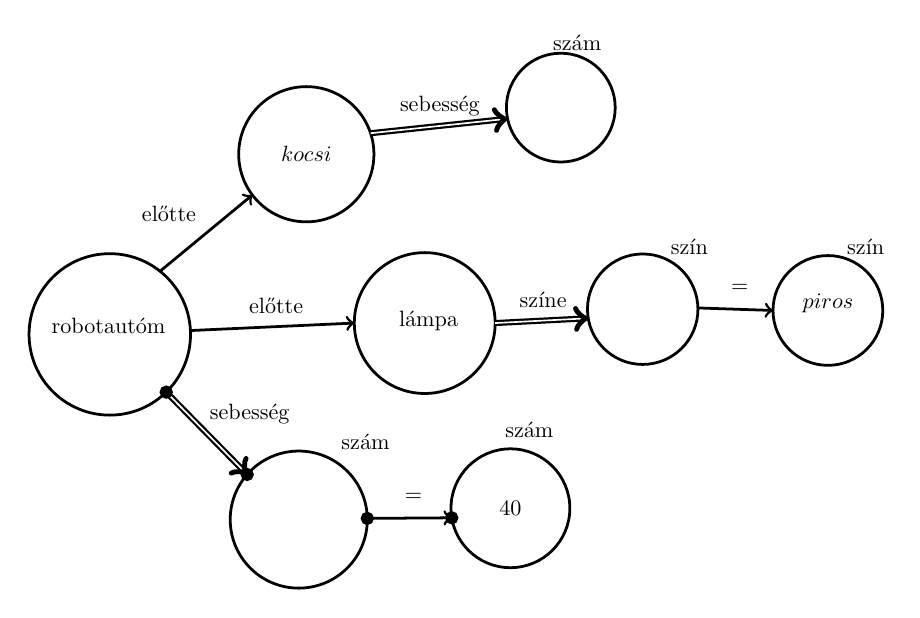
\begin{tikzpicture}[thick,scale=0.8, every node/.style={transform shape}]
\draw [line width=1pt] (-9.5,1.18) circle (1.2815615474880635cm);
\draw [line width=1pt] (-6.38,4.04) circle (1.0733126291998991cm);
\draw [line width=1pt] (-2.34,4.78) circle (0.8637129152675673cm);
\draw [line width=1pt] (-4.5,1.36) circle (1.118033988749895cm);
\draw [line width=1pt] (-1.04,1.58) circle (0.8768124086713191cm);
\draw [line width=1pt] (1.9,1.56) circle (0.8713208364316788cm);
\draw [line width=1pt] (-6.5,-1.76) circle (1.0881176406988353cm);
\draw [line width=1pt] (-3.14,-1.58) circle (0.9433981132056606cm);
\draw [->,line width=1pt] (-8.701912919368261,2.182724793614234) -- (-7.236361075191666,3.3929716320774075);
\draw [->,line width=1pt] (-8.219889003681348,1.2409576664913641) -- (-5.618033988749895,1.36);
\draw [->,double] (-8.604037725755443,0.26367494679534053) -- (-7.3188919774893755,-1.0434695196967962);
\draw [->,line width=1pt] (-5.412049774894232,-1.7409131539455127) -- (-4.071140796172714,-1.7315810598420697);
\draw [->,double] (-5.3598213634935154,4.373519938857889) -- (-3.18539410437372,4.603057047921779);
\draw [->,double] (-3.381966011250105,1.36) -- (-1.9048824322540158,1.435852927957664);
\draw [->,line width=1pt] (-0.16341395312635298,1.5999224101562192) -- (1.028679163568321,1.56);
\draw[color=black] (-9.52,1.31) node {robotaut\'om};
\draw[color=black] (-6.38,4.04) node {$kocsi$};
\draw[color=black] (-2.08,5.81) node {sz\'am};
\draw[color=black] (-4.44,1.39) node {l\'ampa};
\draw[color=black] (1.9,1.67) node {$piros$};
\draw[color=black] (2.5,2.567) node {sz\'in};
\draw[color=black] (-.3,2.567) node {sz\'in};
\draw[color=black] (-5.44,-.53) node {sz\'am};
\draw[color=black] (-2.84,-.333) node {sz\'am};
\draw[color=black] (-3.14,-1.58) node {$40$};
\draw[color=black] (-8.56,3.09) node {el\H otte};
\draw[color=black] (-6.86,1.63) node {el\H otte};
\draw [fill=black] (-8.604037725755443,0.26367494679534053) circle (2.5pt);
\draw [fill=black] (-7.3188919774893755,-1.0434695196967962) circle (2.5pt);
\draw[color=black] (-7.28,-0.09) node {sebess\'eg};
\draw [fill=black] (-5.412049774894232,-1.7409131539455127) circle (2.5pt);
\draw [fill=black] (-4.071140796172714,-1.7315810598420697) circle (2.5pt);
\draw[color=black] (-4.68,-1.41) node {$=$};
\draw[color=black] (-4.26,4.81) node {sebess\'eg};
\draw[color=black] (-2.62,1.73) node {sz\'ine};
\draw[color=black] (0.5,1.91) node {=};
\end{tikzpicture}
\end{tcolorbox}

\begin{prologbox}
sebesseg(robotautom, 40).
maxseb(robotautom, 60).
elotte(robotautom, semmi, 0, 0).
savkozep(robotautom, 6).

gyorsithat(X) :- sebesseg(X, V), maxseb(X, VMAX), V<VMAX.
balrahuz(X) :- savkozep(X, R), R<0.
jobbrahuz(X) :- savkozep(X, R), R>0.
szabadUt(X) :- elotte(X, semmi, 0, 0).

gy(X, Ret) :- gyorsithat(X), !, Ret is 1; Ret is 0.
bh(X, Ret) :- balrahuz(X), !, Ret is 1; Ret is 0.
jh(X, Ret) :- jobbrahuz(X), !, Ret is 1; Ret is 0.
sz(X, Ret) :- szabadUt(X), !, Ret is 1; Ret is 0.

do(X, Akcio) :-
  length(HuzalozottVezerles, 5),
  member(ctrl(1,_,_,1, gyorsits), HuzalozottVezerles),
  member(ctrl(_,1,_,1, jobbraTarts), HuzalozottVezerles),
  member(ctrl(_,_,1,1, balraTarts), HuzalozottVezerles),
  member(ctrl(_,_,_,0, lassits), HuzalozottVezerles),
  gy(X, Ret1),  bh(X, Ret2),  jh(X, Ret3),  sz(X, Ret4),
  member(ctrl(Ret1,Ret2,Ret3,Ret4, Akcio), HuzalozottVezerles).
\end{prologbox}


\section{Esport nyelv}

\section*{License}

{\footnotesize
\begin{verbatim}
% Copyright (C) 2019 Norbert Bátfai
% nbatfa@gmail.com, batfai.norbert@inf.unideb.hu
%
%  This program is free software: you can redistribute it and/or modify
%  it under the terms of the GNU General Public License as published by
%  the Free Software Foundation, either version 3 of the License, or
%  (at your option) any later version.
%
%  This program is distributed in the hope that it will be useful,
%  but WITHOUT ANY WARRANTY; without even the implied warranty of
%  MERCHANTABILITY or FITNESS FOR A PARTICULAR PURPOSE.  See the
%  GNU General Public License for more details.
%
%  You should have received a copy of the GNU General Public License
%  along with this program.  If not, see <https://www.gnu.org/licenses/>.
\end{verbatim}
}

\bibliographystyle{apacite}
\bibliography{prel_para}

\begin{titlepage}
\pagecolor{cyan}
	\centering

	\vspace{1cm}
	{\color{gray!10!white}\Large Ne menjen a tanulás a játék rovására!}
	\\
	\vspace{1cm}
	{\color{black!20!white}\Huge\bf ESPORT NYELV}

\vspace*{\fill}

	{\color{gray!10!white}\Large Don't learn at the expense of gaming.}
	\vspace{1cm}
\\

	{\color{black!20!white}\Huge\bf ESPORTS LANGUAGE}
	\vspace{1cm}
	\end{titlepage}


\end{document}
